 


\section{Q1}
\label{part1}
\begin{enumerate}


\item Save the tweet URIs, and the mapping to the link(s) each tweet contains
- Note: tweets can have more than 1 links

\item For each t.co link, record the HTTP headers all the way to a terminal HTTP status (i.e. chase down all the redirects)

\item How many unique final URIs? How many duplicate URIs?

\item Build a histogram of how many redirects (every URI will have at least 1)
http://en.wikipedia.org/wiki/Histogram
 
\item Build a histogram of HTTP status codes encountered (you will have at least 20000: 10000 301s, and 10000+ more)


\end{enumerate}

\subsection{Solution}

This assignment has been implemented in Python. Following is the detailed report of how this assignment has been done:

\begin{enumerate}

\item To be able to access Twitter's REST API we need the secret keys. I obtained these by registering an app on Twitter's website from my Twitter account.
\item Instead of directly using the Twitter's REST API, I used 'Tweepy' library which is a wrapper to the Twitter's REST API. This makes coding a bit easier.
\item Using the secret keys, get the authentication token from Twitter and use it in the next webservice calls.
\item Twitter has a limitation on the number of times we can access their API within a certain period of time which is 15 minutes. So, to fetch the tweets, I continuously made the webservice calls to fetch the tweets and once the limit got exhausted, I made my program to wait for 15 minutes before making request for the next set of tweets.
\item I saved the Tweet data in a text file in JSON format. The stored information was Tweet id, Tweet text, URLs, Tweet created date
\item To get the final URLs of t.co URLs from Twitter, I used 'Requests' library of Python.
\item For each t.co URL which was stored in file in the previous step, I made a HTTP HEAD request by setting the 'allow redirects' flag to 'True'. 
\item From the response, I stored all the HTTP status codes in one text file and in other text file I stored the final URL and number of redirects required to reach the final URI.
\item Moreover, I calculated and stored the count of unique and duplicate URIs in the third text file.

\end{enumerate}
\newpage

\subsection{Number of URIs Encountered:}

\begingroup
\obeylines
\input{uniqueUrlsCount.txt}
\endgroup

\subsection{Code Listing}
\subsubsection{tweetFetcher.py}

\lstinputlisting[language=Python,breaklines = true,frame=single,caption={Python program to fetch 10,000 Tweets with links}, label=lst:q1-1,captionpos=b,numbers=left,showspaces=false,showstringspaces=false,basicstyle=\footnotesize]{tweetFetcher.py}
\newpage
%\subsection{Results}

\subsubsection{fetchFinalURI.py}
\lstinputlisting[language=Python,breaklines = true,frame=single,caption={Python program to fetch the final URI for each of the t.co URIs from the Listing 1}, label=lst:q1-1,captionpos=b,numbers=left,showspaces=false,showstringspaces=false,basicstyle=\footnotesize]{fetchFinalURI.py}
\newpage

%\verbatiminput{samplelinks.txt}

\subsubsection{Histograms}
\begin{figure}[ht]    
    \begin{center}
        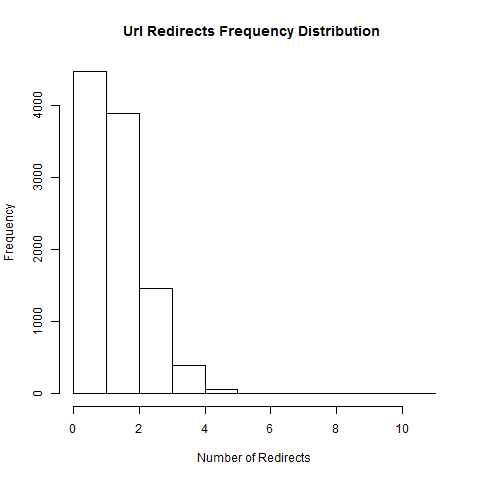
\includegraphics[scale=0.60]{url-redirect-histogram.png}
        \caption{Number of Redirects}
        \label{Number of Redirects}
    \end{center}
\end{figure}

%\newpage
\subsubsection{url-redirect-histogram.R}
\lstinputlisting[language=R,breaklines = true,frame=single,caption={R program to plot histogram for the number of redirects encountered}, label=lst:q2R,captionpos=b,numbers=left,showspaces=false,showstringspaces=false,basicstyle=\footnotesize]{url-redirect-histogram.R}

\newpage
\begin{figure}[ht]    
    \begin{center}
        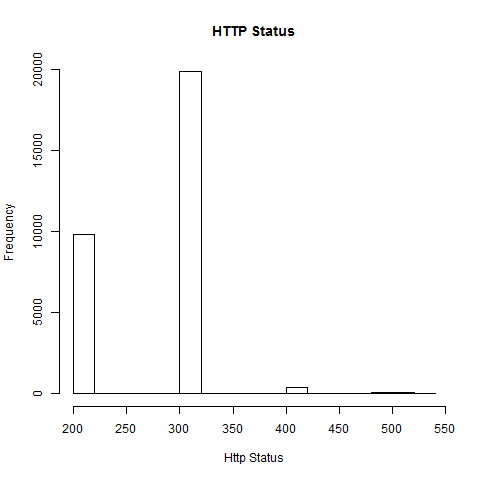
\includegraphics[scale=0.60]{http-statuses.png}
        \caption{HTTP statuses encountered}
        \label{HTTP statuses encountered}
    \end{center}
\end{figure}

%\newpage
\subsubsection{http-statuses.R}
\lstinputlisting[language=R,breaklines = true,frame=single,caption={R program to plot histogram for the HTTP statuses encountered}, label=lst:q2R,captionpos=b,numbers=left,showspaces=false,showstringspaces=false,basicstyle=\footnotesize]{http-statuses.R}
